\documentclass[usenames,dvipsnames]{beamer}


\usepackage{amsmath,amssymb,graphics,graphicx}
%\usepackage{hyperref}
%\usepackage{epigraph}
%\usepackage{mdwlist}
\usepackage{style/preamble}
%\usepackage{hyperref}
\usepackage{color}
\definecolor{mydarkblue}{rgb}{0,0.08,0.45}
\hypersetup{ %
    colorlinks=true,
    linkcolor=mydarkblue,
    citecolor=mydarkblue,
    filecolor=mydarkblue,
    urlcolor=mydarkblue}
\pdfmapfile{+sansmathaccent.map}

\setbeamertemplate{blocks}[rounded][shadow=true]


%%%%%%%%%%%%%%%%%%%%%%%%%%
% Beamer template options
%%%%%%%%%%%%%%%%%%%%%%%%%%

\setbeamertemplate{items}[circle]

%%%%%%%%%%%%%%%%%%%%%%%%%%
% Unused but may be useful in future
%%%%%%%%%%%%%%%%%%%%%%%%%%

\newenvironment{custommargins}[2]%
  {\addtolength{\leftskip}{#1}\addtolength{\rightskip}{#2}}{\par}
  
%%%%%%%%%%%%%%%%%%%%%%%%%%
% Pseudo constants
%%%%%%%%%%%%%%%%%%%%%%%%%%

\newcommand{\standardspace}{
  0.03\textwidth
}

\newcommand{\standardtwocolumnwidth}{
  0.45\textwidth
}

\definecolor{beamerblue}{rgb}{0.2,0.2,0.7}

%%%%%%%%%%%%%%%%%%%%%%%%%%
% Layout
%%%%%%%%%%%%%%%%%%%%%%%%%%

\newcommand{\spacer}[1]{
  \begin{minipage}{#1}
    \hspace{#1}
  \end{minipage}
}

\newcommand{\titlebodyskip}{
  \begin{minipage}[t][\baselineskip][t]{\textwidth}
  \end{minipage}
}

\newcommand{\headerbar}[1]{
  \begin{minipage}[t][2.0\baselineskip][b]{1\textwidth}
    #1
  \end{minipage}
}

\newcommand{\bodyheaderskip}{
	\begin{minipage}[t][\baselineskip][t]{\textwidth}
	\end{minipage}
}

\newcommand{\slidebody}[1]{
  \begin{minipage}[t][0.45\paperheight][t]{\textwidth}
    #1
  \end{minipage}
}

%%%%%%%%%%%%%%%%%%%%%%%%%%
% Slide elements
%%%%%%%%%%%%%%%%%%%%%%%%%%

\newcommand{\frametitleJL}[1]{
  \begin{minipage}[t][2.0\baselineskip][b]{\textwidth}
  {
    \color{beamerblue}
    \large
    #1
  }
  \end{minipage}
}

\newcommand{\columnheader}[2]{
  \begin{minipage}[b]{#1}
  {
  \small
  \begin{center}
    \textbf{#2}
    \end{center}
    \vspace{-2.3\baselineskip}
    \begin{center}
      {\color{beamerblue} \rule{\linewidth}{1pt}}
    \end{center}
  }
  \end{minipage}
}

\newcommand{\columnbody}[2]{
  \begin{minipage}[t][0.45\paperheight][t]{#1}
    \vspace{0.000001\baselineskip}
    {\footnotesize #2}
  \end{minipage}
}

\newcommand{\takeaway}[1]{
  \spacer{0.13\textwidth}
  \begin{minipage}[t][2\baselineskip][c]{0.70\textwidth}
  {
    \small
    \begin{center}
    {
      \color{beamerblue}
      \textbf{#1}
    }	
    \end{center}
  }
  \end{minipage}
  \spacer{0.13\textwidth}
}



\begin{document}

%%%%%%%%%%%%%%%%%%%%%%%%%%%%%%%%%
% Commands to insert agenda slides
%%%%%%%%%%%%%%%%%%%%%%%%%%%%%%%%%

\AtBeginSection{
	\begin{frame}
		\frametitleJL{Agenda}
		\tableofcontents[currentsection]
	\end{frame}
}

\AtBeginSubsection{
	\begin{frame}
		\frametitleJL{Agenda}
		\tableofcontents[currentsubsection]
	\end{frame}
}

%%%%%%%%%%%%%%%%%%%%%%%%%%%%%%%%%
% Title page
%%%%%%%%%%%%%%%%%%%%%%%%%%%%%%%%%

\title{\textbf{Bayesian Interpretations of RKHS Embedding Methods }}
\author{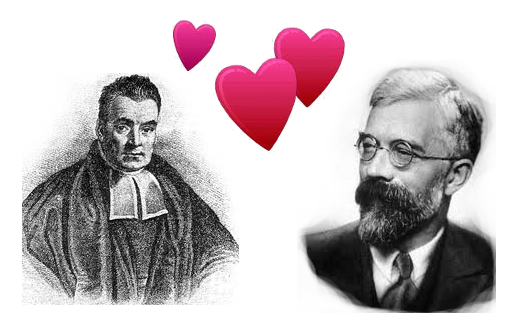
\includegraphics[width=0.6\textwidth]{figures/fisherbayes/lovers2}
\\David Duvenaud} 
 
\institute{Cambridge University
\\Computational and Biological Learning Lab}

\begin{frame}
	\titlepage
\end{frame}

%%%%%%%%%%%%%%%%%%%%%%%%%%%%%%%%%
% Table of contents
%%%%%%%%%%%%%%%%%%%%%%%%%%%%%%%%%

%%%%%%%%%%%%%%%%%%%%%%%%%%%%%%%%%
% Slides
%%%%%%%%%%%%%%%%%%%%%%%%%%%%%%%%%



\begin{frame}[plain, t]
	\frametitleJL{Outline}
	\bodyheaderskip
	\slidebody
	{
		\begin{itemize}
			\item Metrics between distributions
			\begin{itemize}
				\item Maximum Mean Discrepancy
				\item Integrals	under a GP prior
				\item An Equivalence result
			\end{itemize}
			\item Frequentist Methods, Bayesian Takeaways
			\begin{itemize}
				\item Kernel Herding
				\item Hilber-Schmidt Independence Criterion
				\item Kernel Two-sample tests
			\end{itemize}			
			\item Further parallels
			\item Open Questions
		\end{itemize}
	}
\end{frame}



\begin{frame}[plain, t]
	\frametitleJL{Maxmimum Mean Discrepancy}
	%
	\titlebodyskip
	%
%	\bodyheaderskip
	%
%	How to 
	

	\slidebody
	{
		How to measure the difference between two distributions $p(x)$ and $q(x)$?
		
		Maximum Mean Discrepancy.
		
		Assumes function is in a RKHS defined by $k(\cdot , \cdot)$		
		
		Maximum Mean Discrepancy:
		\begin{align*}
			\mmd_{\mathcal{H}}\left(p,q\right) = \sup_{\substack{f\in\He\\\Hnorm{f}=1}}\left\vert\int f(x) p(x) dx - \int f(x) q(x) dx \right\vert
		\end{align*}
	}
	%
%	\takeaway%
%{
%	Takeaway
%}
\end{frame}


\begin{frame}[plain, t]
	\frametitleJL{Bayesian Equivalent}
	%
	\titlebodyskip
	%
%	\bodyheaderskip
	%
%	How to 
	

	\slidebody
	{
		How might a Bayesian measure the difference between two distributions $p(x)$ and $q(x)$?
		
		Answer:  Depends on what for.
		
		Maybe we're expecting to care about difference in population averages of some function of the distribution.  Let's put a 
		
Assuming that $f$ is drawn from a standard GP prior, the expected squared difference in the integral between $f(x)$ against $p(x)$ minus the integral of $f(x)$ against $q(x)$ is equal to the squared Maximum Mean Discrepancy between $p$ and $q$.

\begin{align*}
	\esd_k(p,q) &= \mathbb{E}_{f\sim GP_k} \left( \int f(x) p(x) dx - \int f(x) q(x) dx \right)^2\\
\end{align*}

	}
	%
%	\takeaway%
%{
%	Takeaway
%}
\end{frame}



\begin{frame}[plain, t]
	\frametitleJL{Unification}
	%
	\titlebodyskip
	%
%	\bodyheaderskip
	%
%	How to 
	

	\slidebody
	{
		How to measure the difference between two distributions $p(x)$ and $q(x)$?
		
		Maximum Mean Discrepancy.
		
		Assumes function is in a RKHS defined by $k(\cdot , \cdot)$		
		
		Maximum Mean Discrepancy:
		\begin{align*}
			\mmd_{\mathcal{H}}\left(p,q\right) = \sup_{\substack{f\in\He\\\Hnorm{f}=1}}\left\vert\int f(x) p(x) dx - \int f(x) q(x) dx \right\vert
		\end{align*}
		\pause
		In KH, $p(x)$ is true distribution, and $q(x)$ is a set of point masses around sample locations $\{\vx_1,\ldots,\vx_{N}\}$:
		Assuming function is in a Reproducing Kernel Hilbert Space defined by $k(\cdot , \cdot)$, MMD has closed form.
		\begin{align*}
			\epsilon_{KH}&\left(\{\vx_1,\ldots,\vx_{N}\}\right) & = 
			\mmd_{\He}\left(p, \underbrace{\frac{1}{N}\sum_{n=1}^{N}\delta_{x_n}}_{q(x)}\right) \\
		 	%& = \expectargs{\vx, \vx' \sim p}{k(\vx, \vx')} \\
		 	& = \int \!\!\! \int k(\vx, \vx') p(x) p(x') dx dx' \\
			& \quad -2 \frac{1}{N}\sum_{n=1}^{N}\int k(x,x_n) p(x) dx \\
			& \quad + \frac{1}{N^2}\sum_{n,m=1}^{N} k(x_n,x_m)
		\end{align*}
	}
	%
%	\takeaway%
%{
%	Takeaway
%}
\end{frame}





\begin{frame}[plain, t]
	\frametitleJL{Maxmimum Mean Discrepancy}
	%
	\titlebodyskip
	%
%	\bodyheaderskip
	%
%	How to 
	

	\slidebody
	{
		How to measure the difference between two distributions $p(x)$ and $q(x)$?
		
		Maximum Mean Discrepancy.
		
		Assumes function is in a RKHS defined by $k(\cdot , \cdot)$		
		
		Maximum Mean Discrepancy:
		\begin{align*}
			\mmd_{\mathcal{H}}\left(p,q\right) = \sup_{\substack{f\in\He\\\Hnorm{f}=1}}\left\vert\int f(x) p(x) dx - \int f(x) q(x) dx \right\vert
		\end{align*}
		\pause
		In KH, $p(x)$ is true distribution, and $q(x)$ is a set of point masses around sample locations $\{\vx_1,\ldots,\vx_{N}\}$:
		\begin{align*}
			\epsilon_{KH}&\left(\{\vx_1,\ldots,\vx_{N}\}\right) = 
			\mmd_{\He}\left(p, \underbrace{\frac{1}{N}\sum_{n=1}^{N}\delta_{x_n}}_{q(x)}\right)
		\end{align*}
	}
	%
%	\takeaway%
%{
%	Takeaway
%}
\end{frame}



\begin{frame}[plain, t]
	\frametitleJL{Kernel Herding}
	%
	\titlebodyskip
	%
%	\bodyheaderskip
	%
	%Assumes function is in a RKHS defined by $k(\cdot , \cdot)$	
	\slidebody
	{
	\begin{itemize}
\item 		

\pause

\item When sequentially minimizing MMD, new point is added at:
\begin{align*}
%\nonumber \vx_{n+1} & = \argmin_{\vx \in \mathcal{X}} \mmd \left( p, \frac{1}{N}\sum_{n=1}^{N+1}\delta_{x_n} 5\right) \\
%& = \argmax_{\vx \in \mathcal{X}} 2 \expectargs{\vx' \sim p}{k(\vx, \vx')} \nonumber \\
x_{N+1} = \argmax_{\vx \in \mathcal{X}} \bigg[ 2 \! \int \! k(\vx, \vx') p(x') dx' \nonumber - \frac{1}{N+1}\sum_{m=1}^{N} k(\vx,\vx_m) \bigg]\\
\end{align*}
\end{itemize}
	}
	%
%	\takeaway%
%{
%	Takeaway
%}
\end{frame}




\begin{frame}[plain, t]
	\frametitleJL{Bayesian Quadrature (a.k.a. Bayesian Monte Carlo)}
	%
	\titlebodyskip
	%
	\headerbar
	{
%		\columnheader{\standardtwocolumnwidth}
%		{
%			Simple Monte Carlo
%		}
		%
%		\spacer{\standardspace}
		%
%		\columnheader{\standardtwocolumnwidth}
%		{
%			Simple Monte Carlo
%		}
	}
	%
	\bodyheaderskip
	%
	\slidebody
	{
%		\columnbody{\standardtwocolumnwidth}
%		{	
		{\color{mydarkblue}[O'Hagan, 1987, Rasmussen \& Ghahramani, 2003]	}
			\begin{itemize}
			
			\pause
				\item Places a GP prior on $f$, defined by $k(\cdot, \cdot)$ and a mean function.
				\item Integrating over possible $f$ implies posterior over $Z$.
				
%		}
		%
%		\spacer{\standardspace}
		%
%		\columnbody{\standardtwocolumnwidth}
%		{
%			\vskip10pt
%			\centering
       		\only<2>{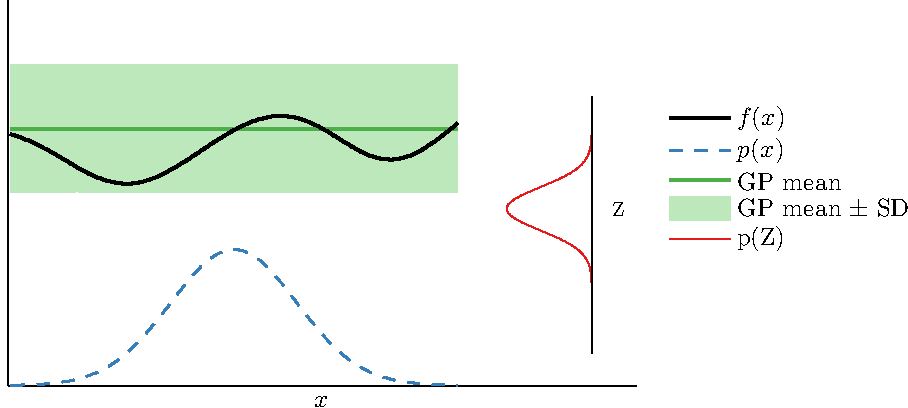
\includegraphics[width=10cm]{figures/bq_buildup/buildup_nosamps0}}
       		\only<3>{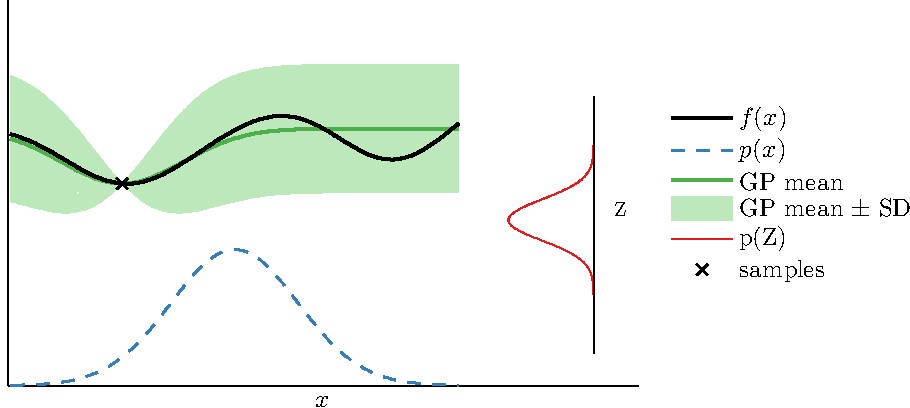
\includegraphics[width=10cm]{figures/bq_buildup/buildup_samps1}}
       		\only<4>{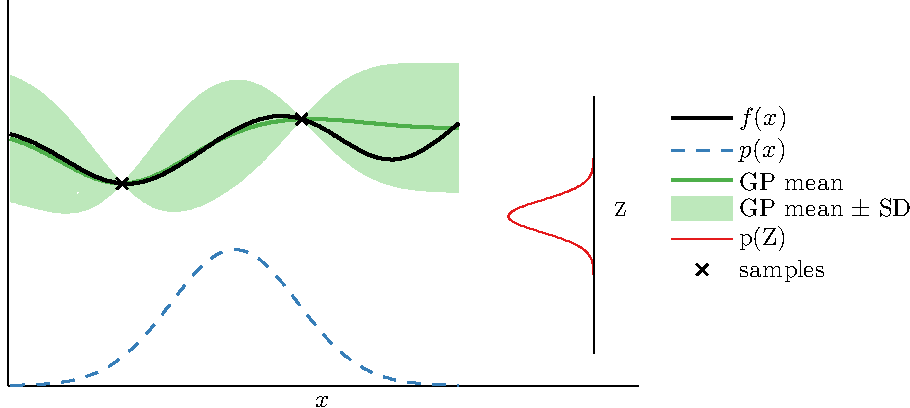
\includegraphics[width=10cm]{figures/bq_buildup/buildup_samps2}}
       		\only<5>{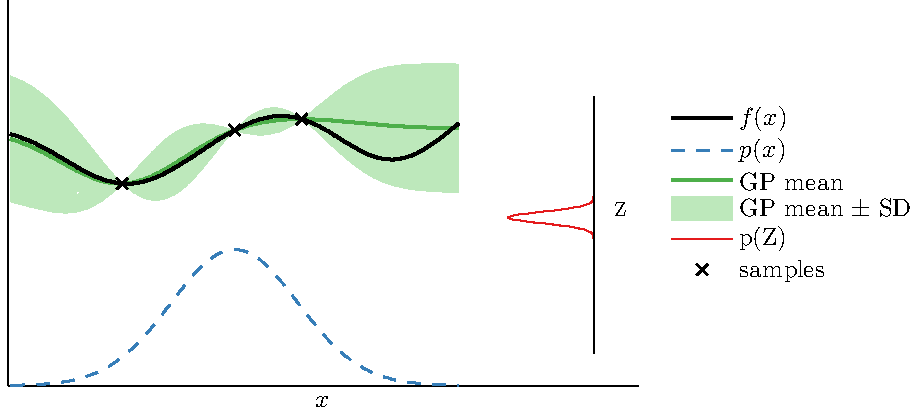
\includegraphics[width=10cm]{figures/bq_buildup/buildup_samps3}}
       		\only<6>{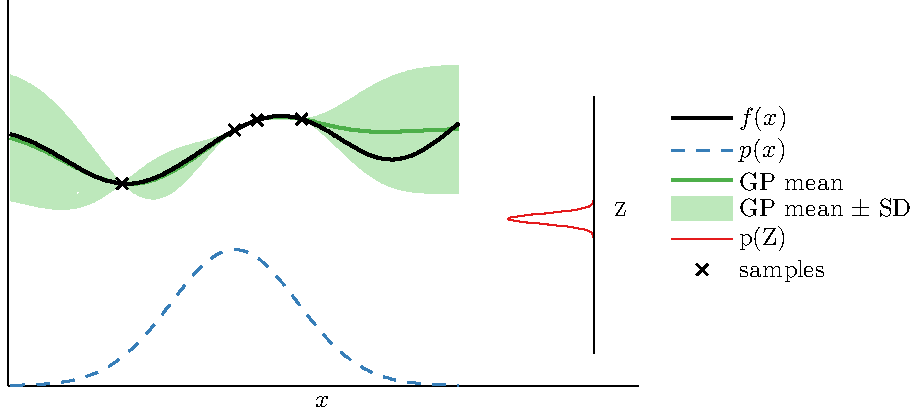
\includegraphics[width=10cm]{figures/bq_buildup/buildup_samps4}}       		      
       		\only<7-8>{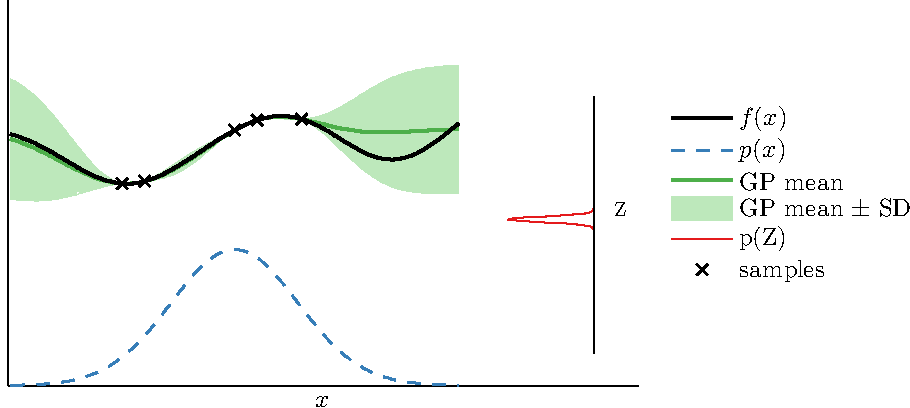
\includegraphics[width=10cm]{figures/bq_buildup/buildup_samps5}}
       		\only<8>{
       		\item Gives flexibility in choosing sample locations.}
			\end{itemize}   		
%		}
	}
	%
%	\takeaway%
%{
%	Takeaway
%}
\end{frame}



\begin{frame}[plain, t]
	\frametitleJL{Bayesian Quadrature Estimator}
	%
	\titlebodyskip
	%
%	\headerbar
%	{
%		\columnheader{\standardtwocolumnwidth}
%		{
%			Expectation of $Z$
%		}
		%
%		\spacer{\standardspace}
		%
%	}
	%
%	\bodyheaderskip
	%
%	\slidebody
%	{
%		\columnbody{\standardtwocolumnwidth}
%		{		

Posterior over $Z$ has mean linear in $f(x_s)$:
\begin{align*}
\expectargs{\gp}{Z|f(x_s)} %& = \expectargs{\gp}{\int f(\vx)p(\vx)d\vx} \\
% & = \int\!\!\! \int\!\! f(\vx) p(\vx) d\vx p(f(\vx)|\vf(\vx_s)) df\\
  & = \sum_{i=1}^N w_{\small{BQ}}^{(i)} \vf(\vx_i)
  \end{align*}
  where
  \begin{align*} 
% & = \int\!\!\! \int\!\! f(\vx) p(\vx) d\vx p(f(\vx)|\vf(\vx_s)) df\\
% & = \int\!\!\! \mf(\vx) p(\vx) d\vx df \\
% & = \left[ \int\!\! k(\vx, \vX) p(\vx) d\vx \right] K^{-1} \vf(\vX) \\
 w_{\small{BQ}} & = \vz^T K\inv \qquad \textrm{and} \qquad z_n = \int\!\! k(\vx, \vx_n) p(\vx) d\vx
\end{align*} 

%\end{align}
%		}
%	}
	%
%	\takeaway%
%{
	%\pause What is relation to herding?
%}
\end{frame}


\begin{frame}[plain, t]
	\frametitleJL{How to select samples?}
	%
	\titlebodyskip
	%
%	\headerbar
%	{
%		\columnheader{\standardtwocolumnwidth}
%		{
%			Expectation of $Z$
%		}
		%
%		\spacer{\standardspace}
		%
%	}
	%
%	\bodyheaderskip
	%
%	\slidebody
%	{
%		\columnbody{\standardtwocolumnwidth}
%		{		
\pause
\begin{itemize}
\item Natural to minimize the posterior variance of $Z$:
%$$\varianceargs{}{Z|f(x_s)} = \expectargs{\vx, \vx' \sim p}{k(\vx, \vx')} - \vz^T K\inv \vz$$
\begin{align*}
\varianceargs{}{Z|f(x_s)} & = \int \! \! \int \! k(\vx, \vx') p(x) p(x') dx dx' - \vz^T K\inv \vz \\
& \textrm{where} \qquad z_n = \int\!\! k(\vx, \vx_n) p(\vx) d\vx
\end{align*}
\pause
\item Favours samples in regions where $p(x)$ is high, but also where covariance with other samples is low.  Similar flavour to herding objective.
\pause
\item Can choose samples sequentially: Sequential Bayesian Quadrature.
\end{itemize}

%		}
%	}
	
%	\takeaway%
%{
%	\pause What is precise relation to herding?
%}
\end{frame}


\definecolor{lightblue}{rgb}{0.9,0.9, 1} 
\setbeamercolor{block title}{bg=blue,fg=white}%bg=background, fg= foreground
\setbeamercolor{block body}{bg=lightblue,fg=black}%bg=background, fg= foreground

\begin{frame}[plain, t]
	\frametitleJL{Relating Objectives}
	%
	\titlebodyskip
	%
%	\headerbar
%	{
%		\columnheader{\standardtwocolumnwidth}
%		{
%			Herding [cite]
%		}
		%
%		\spacer{\standardspace}
		%
%		\columnheader{\standardtwocolumnwidth}
%		{
%			Kernel Herding [cite]
%		}
%	}
	%
%	\bodyheaderskip
	%
 \slidebody
	{
	%	\columnbody{11cm}
	%	{		

		KH and BQ have completely different motivations:
		\begin{itemize}
			\item KH minimizes a worst-case bound
			\item BQ minimizes a posterior variance
		\end{itemize}
		Is there any correspondence?
	\pause
	\begin{block}{First Main Result}
	\begin{align*}
		\varianceargs{}{Z \vert f(x_s)} = \mmd^2(p,q_{\bq{}})
	\end{align*}		

		%How to compare the two?
		%\pause
		
		Where  $$q_{\bq{}}(x) = \sum_{n=1}^{N}w^{(n)}_{\bq{}}\delta_{x_n}(x)$$ 
	\end{block}		
		%under the RKHS defined by the covariance function of GP prior.
%		\pause
%		Then, $\mmd(p, q_{\bq{}})$ is identical to the GP posterior variance:
%The expected variance in the Bayesian quadrature estimate $\varianceargs{}{Z_{f,p}}$ is exactly the squared maximum mean discrepancy between the target distribution $p$ and BQ weighted ``distribution'' $q_{\bq{}}(x) = \sum_{n=1}^{N}w^{(n)}_{\bq{}}\delta_{x_n}(x)$:

	%	}
	}
	\pause
	
	\vspace{0.7in}
%	Frequentist and Bayesian criteria are identical!	

	\takeaway
{
BQ is minimizing KH objective
}
\end{frame}



\begin{frame}[plain, t]
	\frametitleJL{Performance}
	%
	\titlebodyskip
	%
%	\headerbar
%	{
%		\columnheader{\standardtwocolumnwidth}
%		{
%			Herding [cite]
%		}
		%
%		\spacer{\standardspace}
		%
%		\columnheader{\standardtwocolumnwidth}
%		{
%			Kernel Herding [cite]
%		}
%	}
	%
%	\bodyheaderskip
	%
	\slidebody
	{
	%	\columnbody{11cm}
%		{
\begin{itemize}
		\item KH and BQ are minimizing the same objective, but BQ has freedom to choose weights.% So, it can presumably do better.
		\pause
		\item How does this affect performance?
	    \pause 

	\begin{block}{Second Main Result}
	BQ estimator is the optimal weighting strategy:
\begin{align*}
\varianceargs{}{Z\vert f(x_s)} = \inf_{\bm{w}\in\mathbb{R}^N} \sup_{\substack{f\in\He\\\Hnorm{f}{\He}=1}} \left| \int f(x) p(x) dx - \sum_{n=1}^{N}w_n 	f(x_n)\right|^2
\end{align*}
\end{block}
\pause

$\varianceargs{}{Z\vert f(x_s)}$ has two interpretations:
\item Bayesian: posterior variance of Z under a GP prior.
\item Frequentist: tight bound on estimation error of Z.
\end{itemize}
%		}
	}
	%
%	\takeaway%
%{

	
%}
\end{frame}





\begin{frame}[plain, t]
	\frametitleJL{Conclusions}
	%
	\titlebodyskip
	%
	\headerbar
	{
		%\columnheader{\standardtwocolumnwidth}
		%{
	%		About Sampling
%		}
		%
%		\spacer{\standardspace}
		%
%		\columnheader{\standardtwocolumnwidth}
%		{
%			In General
%		}
	}
	%
	\bodyheaderskip
	%
	\slidebody
	{
%		\columnbody{\standardtwocolumnwidth}
%		{
			\begin{itemize}
				\item Posterior variance of Z under GP prior is equivalent to Maximum Mean Discrepancy, a worst case bound.
				\pause
				\item RKHS assumption gives a tight, closed-form upper bound on Bayesian error.
				\pause
				\item BQ has very fast, but unknown convergence rate.
				\pause
				\item The optimal weighted herding strategy is Bayesian quadrature.
%				\begin{itemize}
%					\item BQ has higher complexity than KH ( $\mathcal{O}(N^3)$ versus $\mathcal{O}(N^2)$) but requires fewer samples.
%					\end{itemize}
%				\pause
		%	\end{itemize}	
%		}
		%
%		\spacer{\standardspace}
		%
%		\columnbody{\standardtwocolumnwidth}
%		{
		%	\begin{itemize}
%				\item Bayesian method has a minimax interpretation.
%				\pause
			\end{itemize}					
%		}
	}
	%
	\takeaway%
{
	Thanks!
}
\end{frame}

\bibliographystyle{format/icml2013}
\bibliography{connections}


\end{document}

